\documentclass{beamer}
\usepackage{xcolor}
\usepackage{listings}
\usepackage{graphicx}
\usepackage{amsmath , amsthm , amssymb}


\definecolor{mai_color}{RGB}{153,204,255}
\definecolor{ningen_banzai}{RGB}{128,0,0}
\definecolor{azulft}{RGB}{0,0,128}



\setbeamercolor{background canvas}{bg = mai_color}

\setbeamercolor{block body}{bg=ningen_banzai}


\begin{document}

\lstset{basicstyle = small, breaklines=true, captionpos=b}

    \begin{frame}
        \frametitle{Presentación}
        \Huge\textbf{Proyecto de Programación Moogle}\\
\textcolor{ningen_banzai}{\large Olivia Ortiz Arboláez}
\textcolor{orange}{\tiny Julio de 2023}\\

\vspace{10 pt}
\Large \textcolor{azulft}{\textbf{Moogle!}} Es un proyecto que busca implementar un motor de búsqueda de palabras de archivos \textcolor{orange}{.txt}.
Para esto fue requerido un proceso de investigación sobre ciertas utilidades, fórmulas y la correcta puesta en práctica de estas para conseguir hacer un código en C\# que cumpla este objetivo.\\
\vspace{5 pt}
Dicho esto, comencemos.

    \end{frame}

\begin{frame}
    \frametitle{Inicio}
    \Large En este proyecto fue necesaria la creación de varias clases para tener un código más organizado y entendible a la hora de idearlo. Estas clases se encuentran dentro de MoogleEngine y son:
    \begin{itemize}
        \item \textcolor{purple}{Database}
        \item \textcolor{green!80!black}{Document}
        \item \textcolor{orange}{Vector}
        \item \textcolor{magenta}{Xtra}
    \end{itemize}

\end{frame}

\begin{frame}

    \begin{figure}
        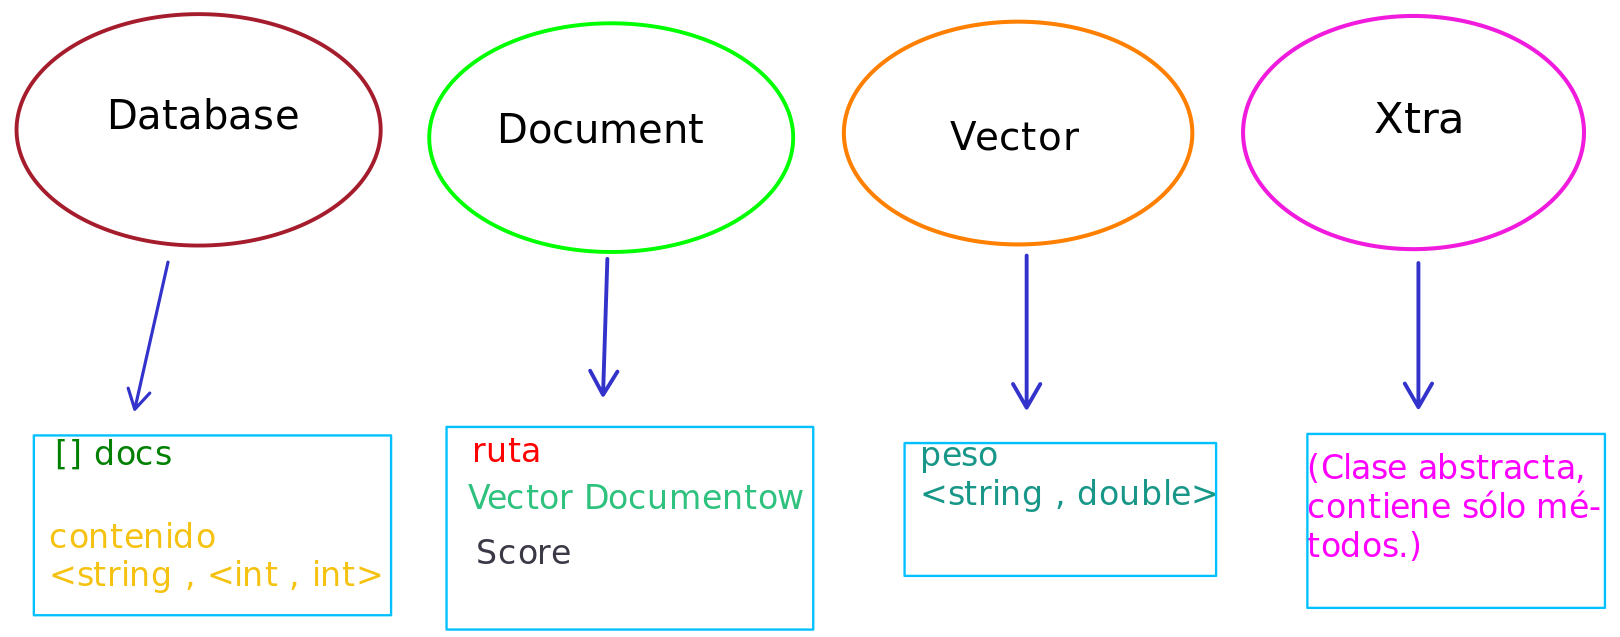
\includegraphics[width = 10 cm , height=6 cm]{./captura1.jpg}
    \end{figure}


\end{frame}

\begin{frame}
    \Large Nuestro programa comienza principalmente en \textcolor{purple}{Database}, creando un nuevo array tipo \textcolor{green}{Document}.
    Todos los objetos tipo \textcolor{green}{Document} tienen la propiedad ruta en dicha clase. Por
tanto el array contendrá constancia de dicha propiedad en cada elemento que
posea. 

\end{frame}

\begin{frame}[fragile]
    Ahora bien, es momento de cargar los documentos. Para ello fue empleada la siguiente función:


\begin{lstlisting}
      private void CargarDocs(string folder)
    {
        IEnumerable <string> Verarchivos = Directory.EnumerateFiles (folder , "*.txt" , SearchOption.AllDirectories) ;
        this.docs = new Document[Verarchivos.Count()] ;
       
        Parallel.For(0 , docs.Length , i => 
        {
            this.docs[i] = new Document(Verarchivos.ElementAt(i)) ;           
        });

    }

\end{lstlisting}

\end{frame}


\begin{frame}
   \Large Esta función no hace más que leer los archivos .txt que se encuentran en la carpeta que se le es pasada por parámetro y, por cada 
archivo que encuentra la función \textcolor{green!40!black}{EnumerateFiles} crea un nuevo objeto tipo documento que es enviado hacia el array docs mediante un bucle.\\
Quedando como elementos de docs[] los archivos .txt que están en la carpeta con su ruta almacenada.

\end{frame}

\begin{frame}[fragile]
    Ahora procedemos a llenar este diccionario:
    \begin{lstlisting}
    public Dictionary <string , Dictionary <int , int> > contenido = new Dictionary <string , Dictionary <int , int> > () ;  
\end{lstlisting}

\Large Emplearemos la siguiente función FillDict para leer las palabras en las rutas de los documentos, estandarizarlas y organizarlas.
Para Estandarizar las palabras usamos una función que está ya implementada en la clase Xtra.

\end{frame}


\begin{frame}[fragile]
    
\begin{lstlisting}
 
    private void FillDict ()
    {
                for (int i = 0; i < docs.Length; i++)
        {
            string[] text = Xtra.Estandarizador( File.ReadAllText( docs[i].ruta)).Split() ;
         

\end{lstlisting}


\end{frame}


\begin{frame}[fragile]

\begin{lstlisting}
    
       
            foreach (string word in text )
            {
                if ( ! this.contenido.ContainsKey(word) )
                {
                    this.contenido.Add( word , new Dictionary <int , int> ()  ) ;
                }


\end{lstlisting}

    
\end{frame}


\begin{frame}[fragile]
    \begin{lstlisting}
     if (! contenido[word].ContainsKey(i) )
                {
                    contenido[word].Add(i , 0);
                }
                
                contenido[word][i]++ ;
            }
        }
    }       
    \end{lstlisting}
\end{frame}


\begin{frame}
        \frametitle{Trabajo con Vectores}
\Large El TF-IDF (\emph{\textbf{en inglés.}Term Frequency - Inverse Document Frequency}) sirve para evaluar la importancia de un término en un documento dentro de un conjunto de documentos.
Lo esencial detrás del TF-IDF es que las palabras que ocurren con frecuencia en un documento, pero raramente en otros documentos, adquieren mayor importancia y son distintivas de ese documento en particular.\\

\end{frame}

\begin{frame}[fragile]
    \Large Para obtener estas propiedades trabajaremos con el diccionario peso de la clase \textcolor{orange}{Vector}.


\begin{lstlisting}
    
public class Vector
{
public Dictionary <string , double> peso = new Dictionary <string ,double> ();

}
\end{lstlisting}


\end{frame}


\begin{frame}

  Las fórmulas que emplearemos para calcular el TF y el IDF son las siguientes:    
\begin{equation} \label{eq:TF}
\textcolor{blue!70!black}{TF  =  \tiny\frac{{\#\quad de\quad veces\quad que\quad el\quad t\acute{e}rmino\quad aparece\quad en\quad el\quad documento}}{{\#\quad de\quad veces\quad est\acute{a}\quad la\quad palabra\quad m\acute{a}s\quad repetida\quad en\quad el\quad documento}}}
\end{equation}    


 \begin{equation}
               \textcolor{violet!100!black} {IDF = \tiny \log \frac{cantidad\quad total\quad de\quad documentos}{cantidad\quad de\quad documentos\quad donde\quad est\acute{a}\quad la\quad palabra} }
            \end{equation}


\end{frame}


\begin{frame}[fragile]
    Mediante la función siguiente tendremos ya cada palabra previamente existente en \textcolor{yellow!80!black}{contenido} almacenada en un diccionario peso:

\begin{lstlisting}
       public void TFIDF (Dictionary<string , Dictionary<int , int>> \textcolor{yellow}{contenido})
    {   
        MaxFrecuency(\textcolor{yellow}{contenido}) ; 
        foreach( string word in \textcolor{yellow}{contenido}.Keys)
        {
            
               
\end{lstlisting}


\end{frame}

\begin{frame}[fragile]
    \begin{lstlisting}
        //formula IDF
            double idf = Math.Log10( (docs.Length +1.0) / (\textcolor{yellow}{contenido}[word].Count() + 1.0 ));
            foreach (int num in \textcolor{yellow}{contenido}[word].Keys)
        {
         //formula TF
                double tf = (double)\textcolor{yellow}{contenido}[word][num] / (docs[num].maxfrec+ 1.0) ;
                
                //Crea los vectores documentos con su TFIDF asociado.
                docs[num].Documentow[word] = tf * idf  ;
                
            }
        }    
    }   




    \end{lstlisting}
    
\end{frame}

\begin{frame}
    
\Large A continuación de esto se hace un procedimiento similar pero con las palabras de la búsqueda del usuario. Se estandarizan estas palabras, se separan y se envían a un array que se le es enviado a una función que halla el TF*IDF de la query.
Para crear este vector query se usan dos funciones más de la clase \textcolor{magenta}{Xtra}, Contar y FrecMAX.


\end{frame}




\begin{frame}[fragile]

\Large Actualmente, contamos con el \textcolor{orange}{Vector Documentow} y el \textcolor{teal}{Vector Query}, que guardan en un diccionario la relación de cada palabra con su peso calculado. ¿Cómo podemos saber qué tan \textbf{\emph{similares}} son estos vectores que tenemos?
Aplicaremos para ello la fórmula de la Similitud del Coseno.
\begin{itemize}
    \item La Similitud del Coseno devuelve un valor que se encuentra entre -1 y 1.
    \item Un  resultado de -1 en este caso al calcularla, no es posible, puesto que trabajamos sólo con los casos en que esté o no esté la palabra.

\end{itemize}

    
\end{frame}

\begin{frame}
\begin{itemize}
    \item \Large Mientras más cercano sea el resultado a 0, indica que son diferentes los vectores o no tienen relación alguna.
    \item Mientras más cercano sea el resultado a 1 de calcular la Similitud del Coseno, mayor será la similitud entre ambos.
\end{itemize}    

Entonces, sea dicha fórmula la siguiente:

\begin{equation}
    \frac{\sum_{\vec{\vec{\delta}}  *  \vec{\vec{\nu}} } } {|\vec{\delta} | * |\vec{\nu} |} 
\end{equation}
\begin{equation}\vec{\delta}\quad vector\quad query\quad y\quad \vec{\nu}\quad vector\quad Documento \end{equation}

Lo presente en el numerador de esta fórmula es llamado producto escalar de ambos vectores y se obtiene multiplicando cada elemento del vector \textcolor{teal}{query} por su correspondiente en el vector \textcolor{orange}{Documentow}. 


\end{frame}

\begin{equation}
\vec{\delta}_{1} * \vec{\nu}_{1} + \vec{\delta}_{2} * \vec{\nu}_{2}  
\end{equation}    

Para calcular lo que se halla en el denominador de la fórmula, que es denominado ¨Normas de Vectores¨, en el Proyecto se utiliza un método llamado Norma de la clase \textcolor{magenta}{Xtra}. La fórmula general para hallar la norma es:
\begin{equation}
    \sqrt{\vec{\nu}_{1}^2 + \vec{\nu}_{2}^2 + \vec{\nu}_{3}^2 } 
\end{equation}

\begin{frame}[fragile]
Teniendo todo esto en cuenta, se empleó el siguiente método SimilitudVect de la clase \textcolor{pink}{Vector} :
\begin{lstlisting}
     public static double SimilitudVect (Dictionary <string , double> Documentow , Dictionary <string , double> quervector)
    {
        double Escalar = 0.0;
        foreach (string word in quervector.Keys)
        {
                if (Documentow.ContainsKey(word))
                {
                    Escalar += quervector[word] * Documentow[word];
                }
       

\end{lstlisting}

\end{frame}    


\begin{frame}[fragile]

       \begin{lstlisting}  
        }
        return Escalar / (Vector.Norma(Documentow) * Vector.Norma(quervector)) ;
       }
        \end{lstlisting}


Este resultado se guarda en una propiedad \textcolor{green}{Document} llamada Score mediante un bucle.

        
    \end{frame}

\begin{frame}[fragile]
    \frametitle{Devolver Resultados}
\Large Dentro de la propiedad Score tenemos varios valores, conforme sean más cercanos a 1, el documento asociado al valor más alto será el que tenga mayores coincidencias respecto a la búsqueda, y así sucesivamente. Por lo cual hace falta organizar estos valores de mayor a menor, y así poder llamarlos.
Usando el algoritmo Selection Sort pero adaptado al docs [], que es un array tipo \textcolor{green}{Document}, se consiguió este propósito.

\end{frame}

\begin{frame}[fragile]

\begin{lstlisting}
     public static void SelectionSort(Document [] array)
    {
        int n = array.Length;
        for (int i = 0; i < n - 1 ; i++)
        {
         int Maxindice = i;
         for (int j = i + 1; j < n; j++)
         {
          
\end{lstlisting}

\end{frame}    

\begin{frame}[fragile]
    \begin{lstlisting}
        
    
    if(array[j].Score > array[Maxindice].Score)
          {
            Maxindice = j;
          }  
         } 
         Document temporal = array[Maxindice] ;
         array[Maxindice] = array[i] ;
         array[i] = temporal ; 
        }
    }
\end{lstlisting}

\end{frame}

\Large Ahora con los resultados de mayor valor ordenados, se emplea un bucle para devolver los primeros. Una vez hecho esto el código está listo para ser ejecutado, Solamente ha de realizar una consulta en la barra de búsqueda.

\vspace{1 cm}
\begin{figure}
        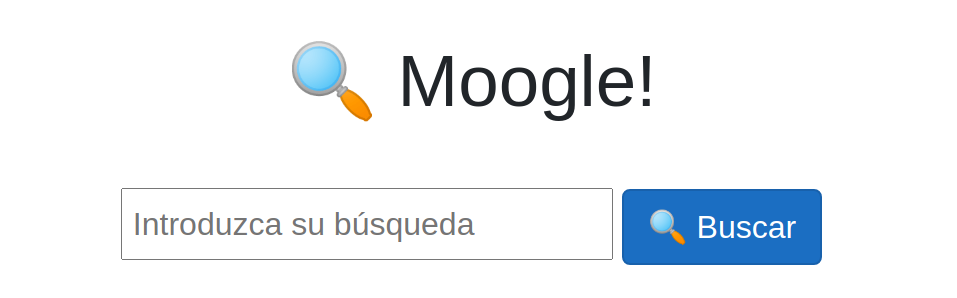
\includegraphics[width = 10 cm ]{./moogle.png}
    \caption{Barra de búsqueda}
    \end{figure}

\end{document}



